\documentclass{beamer}
\usepackage[bahasa]{babel}

% \usepackage{lipsum}
\usepackage{graphicx}
\usepackage{apacite}
\usetheme{Madrid} 
\begin{document}

\begin{frame}
    \huge SPK Olist dataset\\
    Prediksi Review\\ 
    (Ilman samhabib 91122010)
    
\end{frame}

\begin{frame}
    Dataset yang dipakai adalah data penjualan e-commerce oleh perusahaan E-commerce Brazil
\end{frame}


\begin{frame}
    \begin{itemize}
        \item mengisi null/nilai kosong
        \item membuang row yang tidak perlu
        \item menyatukan data yang perlu
        \item menyederhanakan waktu tempuh, fitur:'time to get'
    \end{itemize}
\end{frame}

\begin{frame}
    Di sini akan diperkirakan berapa review yang akan didapatkan, berdasar pada harga,lama sampai, biaya pengiriman...disini diharapkan akan ada model yang cukup baik memprediksi tingkat review yang akan didapatkan berdasar pada fitur tertentu
\end{frame}

\begin{frame}
\frametitle{Korelasi Antar Fitur}
\graphicspath{ {./images/} }
\begin{figure}
\centering
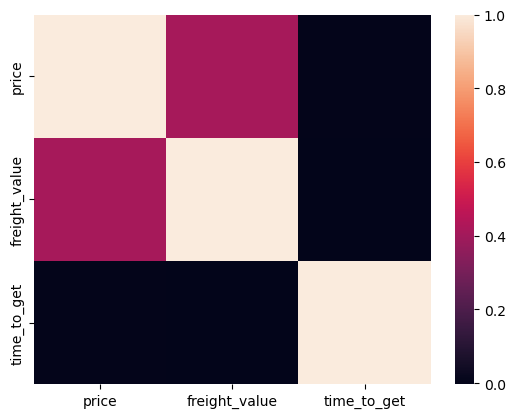
\includegraphics[width=0.8\textwidth]{correlation.png}
\end{figure}
\end{frame}

\begin{frame}
    korelasi antar fitur rendah, fitur fitur tersebut tidak saling berketergantungan 
\end{frame}

\begin{frame}
    beberapa model pengklasifikasian akan dipilih auntuk memprediksi skor review\dots
    \begin{itemize}
        \item K-NN (5 categories,uniform)
        \item XGboost
        \item Random Forest
        \item Decision Tree
    \end{itemize}
    Dataset dibagi menjadi Train dan Test set, dengan test data sebesar 30\%
\end{frame}

\begin{frame}
    \frametitle{k-NN Classifier}
    \graphicspath{ {./images/} }
    \begin{figure}
    \centering
    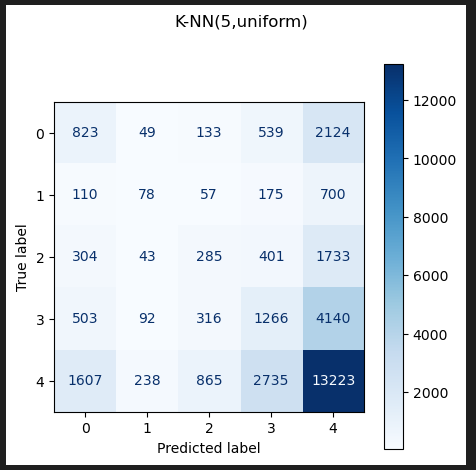
\includegraphics[width=0.6\textwidth]{knn-confusion.png}
    \end{figure}
\end{frame}


\begin{frame}
    \frametitle{Decision Tree Classifier}
    \graphicspath{ {./images/} }
    \begin{figure}
    \centering
    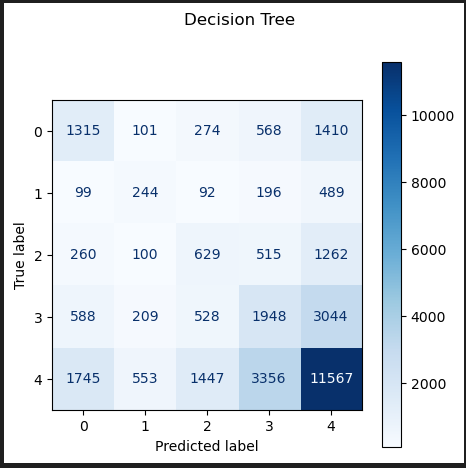
\includegraphics[width=0.6\textwidth]{Dt-confusion.png}
    \end{figure}
\end{frame}

\begin{frame}
    \frametitle{Random Forest Classifier}
    \graphicspath{ {./images/} }
    \begin{figure}
    \centering
    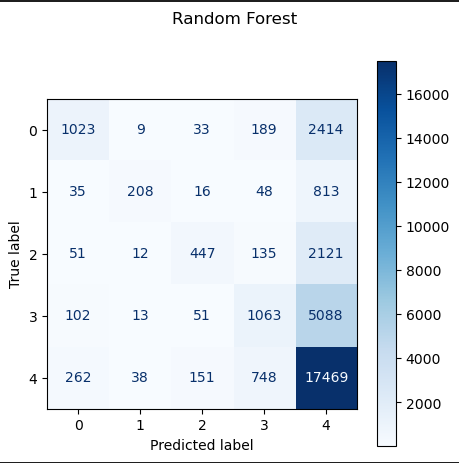
\includegraphics[width=0.6\textwidth]{rf-confusion.png}
    \end{figure}
\end{frame}

\begin{frame}
    \frametitle{XGB Classifier}
    \graphicspath{ {./images/} }
    \begin{figure}
    \centering
    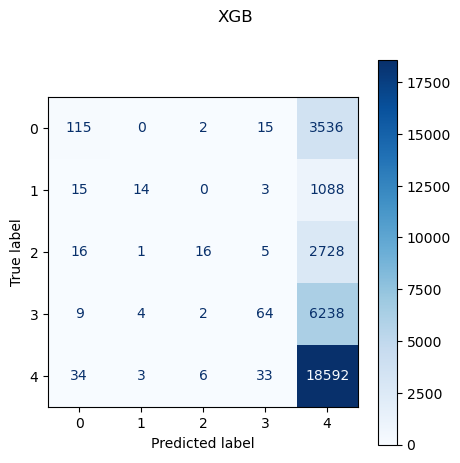
\includegraphics[width=0.6\textwidth]{xgb-confusion.png}
    \end{figure}
\end{frame}

\begin{frame}
    Ke empat model ini memberi prediksi yang cukup baik untuk kategori 5(4) bintang. 
    Tetapi tidak terlalu baik untuk selain 5 bintang  tidak terlalu akurat, ini mungkin disebabkan oleh data yang \emph{imbalance}, mungkin diperlukan penyeimbangan data seperti teknik \emph{oversampling} ataupun \emph{undersampling} ataupun \emph{feature engineering}
\end{frame}



\end{document}
